\documentclass[11pt]{beamer}
\usepackage[T1]{fontenc}
\usepackage[utf8]{inputenc}
\usepackage{babel}[spanish]

\usepackage{pgf,pgfpages}

\usepackage{tikz}
\usetikzlibrary{arrows,shapes,backgrounds,calc}

\usepackage{graphicx}
\usepackage{colortbl}
\usepackage{units}

% \usepackage{calrsfs}
% \DeclareMathAlphabet{\pazocal}{OMS}{zplm}{m}{n}
% \usepackage{calligra}
\usepackage[cal=boondox]{mathalfa}
% \usepackage{bickham}
% \usepackage{boondox-cal}
% \usepackage{boondox-calo}
% \usepackage{dutchcal}

%% Beamer style >>>>>>>>>>>>>>>>>>>>>>>>>
\mode<presentation>
{
  \usetheme{PHD}
  \setbeamercovered{transparent}
  \setbeamertemplate{items}[square]
}

%\usefonttheme[onlymath]{serif}

\beamertemplatenavigationsymbolsempty

\defbeamertemplate{enumerate item}{mycircle}
{
  %\usebeamerfont*{item projected}%
  \usebeamercolor[bg]{item projected}%
  \begin{pgfpicture}{0ex}{0ex}{1.5ex}{0ex}
    \pgfcircle[fill]{\pgfpoint{-0.1pt}{.65ex}}{1.1ex}
    \pgfbox[center,base]{\color{PHDyellow}{\insertenumlabel}}
  \end{pgfpicture}%
}
[action]
{\setbeamerfont{item projected}{size=\scriptsize}}
\setbeamertemplate{enumerate item}[mycircle]

%<<<<<<<<<<<<< beamer style

\title[Matemáticas: pasado $\to$ futuro]{Matemáticas: una visión al pasado para determinar el futuro}
\subtitle{\scriptsize{\color{gray}TFG: Métodos de Galerkin discontinuos para la resolución numérica de EDP}\vspace{-0.9em}}
\author[Daniel Acosta Soba]{\em Daniel Acosta Soba\vspace{-0.9em}} \date{\footnotesize\structure{\em
    Tutor: J. Rafael Rodr\'iguez Galv\'an} \\[1ex] Cádiz, 18 de enero de 2021}

% XeLaTeX font choosing
% \usepackage{fontspec}%{xltxtra} %fontspec}
% \setsansfont{Fontin Sans}
% \setsansfont{Lato}

% PDFLaTeX font choosing
\usepackage[default, scale=1.0]{lato}

\setbeameroption{hide notes} % Only slides
% \setbeameroption{show only notes} % Only notes
% \setbeameroption{show notes on second screen=right} % Both

% Different math fonts, see http://tug.org/pracjourn/2006-1/hartke/hartke.pdf
%\usepackage{eulervm}
%\usepackage{ccfonts, eulervm}
%\usepackage[math]{kurier}
%\usepackage[math]{anttor}
%\usepackage{pxfonts}
%\usepackage{mathpazo}
%\usepackage{mathpple}
%\usepackage[varg]{txfonts}
%\usepackage{arev}
%\usepackage{fourier}

\usepackage{tabularx}
\usepackage{array, multirow, booktabs, rotating} % booktabs: toprule, midrule...

\newcommand{\heatProblem}{(Heat-Problem)\xspace}
\newcommand{\poissonProblem}{(Poisson-Problem)\xspace}

\usepackage{estilo_Rafa}

\theoremstyle{plain}% default
\newtheorem{teorema}{Teorema}
\newtheorem{proposicion}{Proposici\'on}
\newtheorem{lema}{Lema}
\newtheorem{corolario}{Corolario} 
\newtheorem{observacion}{Observaci\'on}

\theoremstyle{definition}
\newtheorem{definicion}{Definici\'on}
\newtheorem{ejemplo}{Ejemplo}
\newtheorem{problema}{Problema} 

\theoremstyle{remark}
\newtheorem*{nota}{Nota}

% Presentation goodies >>>>>>>>>>>>>>>>>>>>>>>>>>>>
\newcommand<>{\myframed}[1]{\alt#2{\tikz[phd] \node[box] {#1};}{{#1}}}
\newcommand<>{\myframedAlert}[1]{\alt#2{\tikz[phdB] \node[boxB] {\color{black}#1};}{{#1}}}
\newcommand<>{\framedmath}[1]{%
\alt#2{\tikz[phd] \node[box] {\ensuremath{#1}};}{\ensuremath{#1}}}
\newcommand{\framedB}[1]{\tikz[phd] \node[boxB] {#1};}
\newcommand{\framedmathB}[1]{\framedB{\ensuremath{\displaystyle{#1}}}}
\newcommand{\ver}[1]{\footnote{See #1}}
\newcommand{\cita}[1]{{\color{PHDgray}\cite{#1}}}
\newcommand\cellalert[2]{\only<#1>{\cellcolor{PHDyellow}}\alt<#1>{\textbf{#2}}{#2}}
\newcommand{\soften}[1]{{\color{PHDgray}#1}}
\newcommand{\rowalert}[7]{%
    \cellalert{#1}{#2} & \cellalert{#1}{#3} &
    \cellalert{#1}{#4} & \cellalert{#1}{#5} &
    \cellalert{#1}{#6} & \cellalert{#1}{#7}}

\newcommand{\kk}{\Delta t}
% \usepackage{wasysym}
% \newcommand{\good}{{\color{PHDgreen}$\CIRCLE$}} %\blacksmiley
% \newcommand{\bad}{{\color{PHDred}$\CIRCLE$}}
\usepackage{pifont}
\newcommand{\good}{{\color{PHDgreen}\ding{52}}}
\newcommand{\bad}{{\color{PHDred}\ding{56}}}
\newcommand{\exclamation}{{\large\color{PHDred}{\textbf{\itshape !}}}}
\newcommand{\question}{{\large\color{PHDred}{\textbf{\itshape ?}}}}
\newcommand\colorUnderLine[2][PHDyellow]{\color{#1}\underline{{\color{black}#2}}\color{black}\xspace}
\newcommand\gris{\color{PHDgray}}
\newcommand\amarillo{\color{PHDyellow}}
\newcommand\tiragris[1]{{\par\hfill\small\gris{#1}}}
%<<<<<<<<<<<<<<<

\setcounter{tocdepth}{2}


%
% Bibliography
%
%\usepackage{natbib}

% To list each bibliographic entry in a line
\setbeamertemplate{bibliography entry title}{}
\setbeamertemplate{bibliography entry location}{}
\setbeamertemplate{bibliography entry note}{}

% ... end of preamble.

\defbeamertemplate*{section page}{mine}[1][\alert{Secci\'on \thesection}]{%
	\begin{centering}
		{\usebeamerfont{section name}\usebeamercolor[fg]{section name}#1}
		\vskip1em\par
		\begin{beamercolorbox}[sep=12pt,center]{part title}
			\usebeamerfont{section title}\insertsection\par
		\end{beamercolorbox}
	\end{centering}
}
\renewcommand*{\sectionpage}{\usebeamertemplate*{section page}}

\defbeamertemplate*{subsection page}{mine}{%
	\begin{centering}
		\vskip1em\par
		\begin{beamercolorbox}[sep=12pt,center]{subsection}
			\usebeamerfont{subsection title}\insertsubsection\par
		\end{beamercolorbox}
	\end{centering}
}

\defbeamertemplate*{subsubsection page}{mine}{%
	\begin{centering}
		\vskip1em\par
		\begin{beamercolorbox}[sep=12pt,center]{subsubsection}
			\usebeamerfont{subsection title}\insertsubsubsection\par
		\end{beamercolorbox}
	\end{centering}
}
\renewcommand*{\sectionpage}{\usebeamertemplate*{section page}}
\renewcommand*{\subsectionpage}{\usebeamertemplate*{subsection page}}
\newcommand{\subsubsectionpage}{\usebeamertemplate{subsubsection page}}
\AtBeginSection{\frame{\sectionpage}}
\AtBeginSubsection{\frame{\subsectionpage}}
\AtBeginSubsubsection{\frame{\subsubsectionpage}}



\renewcommand{\vv}{v}
\renewcommand{\VV}{V}

%-------------------------- MIS PAQUETES -------------------------------

\usepackage{amssymb}
\usepackage{mathrsfs}
\usepackage{mathtools}
\usepackage{subcaption}
\usepackage{multicol}
\usepackage{arydshln} % Líneas discontinuas en tablas
\usepackage{hhline} % Dobles líneas horizontales
%\usepackage{footnote}
%\usepackage{multimedia}

\usepackage{caption}
\captionsetup[table]{name=Cuadro}
\captionsetup[figure]{name=Figura}

\usepackage{pgfplots}

%--------------------------- MIS MACROS --------------------------------


\def\R{\ensuremath{\mathbb R}}
\def\K{\ensuremath{\mathbb K}}
\def\C{\ensuremath{\mathbb C}}
\def\N{\ensuremath{\mathbb N}}
\def\Z{\ensuremath{\mathbb Z}}
\def\Q{\ensuremath{\mathbb Q}}
\def\A{\ensuremath{\mathbb A}}

\def\centra#1{\begin{center} #1\end{center}}

\def\sen{\mathop{\rm sen}\nolimits}
\def\arcsen{\mathop{\rm arcsen}\nolimits}
\def\tg{\mathop{\rm tg}\nolimits}
\def\cotg{\mathop{\rm cotg}\nolimits}
\def\cosec{\mathop{\rm cosec}\nolimits}
\def\arctg{\mathop{\rm arctg}\nolimits}

\def\suma#1#2{\displaystyle\sum_{#1}^{#2}}
\def\fra#1#2{\displaystyle {#1\over #2}}
\def\Lim{\ensuremath{\displaystyle\lim}}

\newcommand{\be}{\begin{enumerate}}
\newcommand{\ee}{\end{enumerate}}

\newcommand{\bi}{\begin{itemize}}
\newcommand{\ei}{\end{itemize}}

\newcommand{\bd}{\begin{description}}
\newcommand{\ed}{\end{description}}

\newcommand{\beq}{\begin{equation}}
\newcommand{\eeq}{\end{equation}}

\newcommand{\braya}{\begin{itemize}\renewcommand{\labelitemi}{\labelitemii}}
\newcommand{\eraya}{\end{itemize}}

\newcommand{\bletra}{\begin{list}{(\alph{enumiii})}{\usecounter{enumiii}}}
\newcommand{\eletra}{\end{list}}

\newcommand{\broman}{\begin{list}{(\roman{enumiii})}{\usecounter{enumiii}}}
\newcommand{\eroman}{\end{list}}

\newcommand{\bRoman}{\begin{list}{(\Roman{enumi})}{\usecounter{enumi}}}
\newcommand{\eRoman}{\end{list}}

\def\xn{(x_1,x_2,\ldots ,x_n)}
\def\yn{(y_1,y_2,\ldots ,y_n)}
\def\xm{(x_1,x_2,\ldots ,x_m)}
\def\ym{(y_1,y_2,\ldots ,y_m)}

\def\caja{\hspace*{\fill}$\Box$}

\def\nveces#1{\matrix{\mathop{\frown}\limits^{#1}
\cr \cdots\cr \mbox{}} }

\def\Veces#1{\buildrel {\buildrel #1\over\frown} \over\cdots}

\def\sucesion#1#2{\left(#1_#2\right)_#2}



%--------------------------- MIS MACROS --------------------------------

\def\escalar#1#2{\left(#1,#2\right)}
\def\dualD#1#2{{\langle #1, #2 \rangle}_{\mathscr{D'},\mathscr{D}}}
\def\escalarL#1#2{\escalar{#1}{#2}_{L^2(\Omega)}}
\def\escalarLd#1#2{\escalar{#1}{#2}_{\left(L^2(\Omega)\right)^d}}
\def\dualH#1#2{\langle#1,#2\rangle_{(H^1(\Omega))',H^1(\Omega)}}

\def\norma#1{\left\|#1\right\|}
\def\normaL#1{\norma{#1}_{L^2(\Omega)}}
\def\normaLd#1{\norma{#1}_{\left(L^2(\Omega)\right)^d}}
\def\normaLinf#1{\norma{#1}_{L^\infty (\Omega)}}
\def\seminorma#1{\left|#1\right|}
\def\salto#1{\left[\!\left[#1\right]\!\right]}
\def\media#1{\left\{\!\!\left\{#1\right\}\!\!\right\}}
\def\uex{u_{\text{ex}}}

\def\D{\mathscr{D}}
\def\T{\mathcal{T}}
\def\E{\mathcal{E}}
\def\S{\mathcal{S}}

\def\asip#1#2{a_h^{\text{sip},\sigma}(#1,#2)}
\def\normasip#1{\norma{#1}_{\text{sip}}}
\def\seminormasalto#1{\left|#1\right|_{\text{s}}}
\def\escalarsip#1#2{\escalar{#1}{#2}_\text{sip}}

\def\acf#1#2{a_h^{\text{cf}}(#1,#2)}
\def\normacf#1{\norma{#1}_{\text{cf}}}
\def\escalarcf#1#2{\escalar{#1}{#2}_\text{cf}}

\def\aupw#1#2{a_h^{\text{upw}}(#1,#2)}
\def\normaupw#1{\norma{#1}_{\text{upw}}}
\def\escalarupw#1#2{\escalar{#1}{#2}_\text{upw}}

\def\adg#1#2{a_h^{\text{DG}}(#1,#2)}

\begin{document}
% Tikz style and beamer template ------->>>
\tikzstyle{every picture}+=[remember picture]
\tikzstyle{na} = [baseline=-.5ex]
\tikzstyle{phd} = [baseline=-.6ex,
  box/.style={rectangle, draw=PHDblueC, thick, fill=PHDblueA,
    align=center, rounded corners, minimum height=1.6em},
  boxB/.style={rectangle, draw=PHDredA, thick, fill=PHDblueA,
    align=center, rounded corners, minimum height=1.6em}]
\tikzstyle{phdB} = [baseline=-.7ex,
  box/.style={rectangle, draw=PHDblueC, thick, fill=PHDblueA,
    align=center, rounded corners, minimum height=1.6em},
  boxB/.style={rectangle, draw=PHDredA, thick, fill=PHDblueA,
    align=center, rounded corners, minimum height=1.6em}]
\tikzstyle{myarrow} = [->,>=latex, PHDredA, shorten >=4pt,
  opacity=.6, line width=0.6mm]
\tikzstyle{myarrow2} = [->,>=latex, PHDblueC, shorten >=4pt, opacity=.2, line width=0.4mm]
\tikzstyle{myarrow3} = [
     opacity=.7,
%    >=triangle 60,              % Nice arrows; your taste may be different
    node distance=6mm and 60mm, % Global setup of box spacing
    every join/.style={norm},   % Default linetype for connecting
                                % boxes
    line width=0.6mm,
    PHDredA,
    ->
    ]
\setbeamertemplate{background}
 {
\includegraphics[width=\paperwidth,height=\paperheight]{frontpage_bg}}
\setbeamertemplate{footline}[default]
% <<<-------


% Write custom titlepage ------->>>
\begin{frame}
  \titlepage
  \vspace{5cm}
\end{frame}

% Write all of the slides..........
\setbeamertemplate{background}{
\includegraphics[width=\paperwidth,height=\paperheight]{slide_bg}}

\begin{frame}{Índice}
  \tableofcontents
\end{frame}

% Start inserting infoline at the end
\setbeamertemplate{footline}[PHDtheme]
% <<<-------

\newcommand{\imgdir}{Undefined, use renewcommand!}


\section{Modelización matemática mediante EDP}

\begin{frame}{Modelización matemática mediante EDP}
	\begin{center}
		\begin{tikzpicture}[
		% Define standard arrow tip
		>=stealth',
		% Define style for boxes
		punkt/.style={
			rectangle,
			rounded corners,
			scale=1.1, fill=gray!20,
			draw=black, very thick,
			text width=6.5em,
			minimum height=2em,
			text centered},
		% Define arrow style
		pil/.style={
			->,
			very thick,
			color=black!75!blue,
			shorten <=2pt,
			shorten >=2pt},
		% line width=1.2pt
		]
		\node[punkt] (A) at (0,0) {\color{PHDgreen}\em Observaciones de un fenómeno};
		\node[punkt] (B) at (6,0) {\color{PHDred}\em Modelo matemático}
		edge[pil, <-, bend left=-45] node[above] {\footnotesize
			\begin{tabular}{l}Leyes de la naturaleza\end{tabular}} (A);
		\node[punkt] (C) at (3,-3) {\color{orange}\em Simulación en ordenador}
		edge[pil, ->, bend left=45]  node[left] {\footnotesize
			\begin{tabular}{l} $\bullet$ Validación\\$\bullet$ Predicción\end{tabular}} (A)
		edge[pil, <-, bend left=-45, inner sep=1.0ex, align=right] node[right] {\footnotesize
			\begin{tabular}{l} $\bullet$ Análisis\\$\bullet$ Aproximación numérica \\
			$\bullet$ Algoritmos\end{tabular}} (B);
		% \path[line width=1.2pt, ->] (A) edge (B);
		% \path[line width=1.2pt, ->] (B) edge (C);
		% \path[line width=1.2pt, ->] (C) edge (A);
		\end{tikzpicture}
	\end{center}
\end{frame}

\subsection{Modelos del clima}

\begin{frame}{Modelos del clima}
	\begin{minipage}{0.55\linewidth}
		\vspace{0.3em}
		\begin{flushright}
			\onslide<1->{\color{darkgray}\small\emph{¿Cómo se comportan los fluidos que forman <<\structure{\bfseries atmósfera}>> y <<\structure{\bfseries océanos}>>?}}
		\end{flushright}
		\vspace{0.3em}
		\onslide<2->{
			\begin{flushright}
				{Modelo matemático (simplificado)
					\color{darkgray}\scriptsize(ecuaciones de
					Navier-Stokes)}
			\end{flushright}
			\begin{block}{}
				\vspace*{-0.4cm}
			\begin{equation*}
			\left\{
			\begin{aligned}
			\frac{\partial \alert<4>{\mathbf{u}}}{\partial t}
			+ (\mathbf{\alert<4>u}\cdot\nabla)\mathbf{\alert<4>u}
			- \nu \Delta \mathbf{\alert<4>u}
			+ \nabla \alert<3>p &= \mathbf{f},
			\\
			\nabla\cdot \mathbf{\alert<4>u} &= 0.
			\end{aligned}
			\right.
			\end{equation*}
			\end{block}
		}
		\vspace{0.1em}
		\begin{flushleft}
			\begin{itemize}
			\item<3>\myframed{Presión atmosférica}
			\\[0.3em]
			\item<4>\myframed{Velocidad del fluido}
			\\[0.3em]
			\item<5>Análisis del modelo:
			\\[0.3em]
			\end{itemize}
		\end{flushleft}
	\end{minipage}
	\hfill
	\begin{minipage}{0.40\linewidth}
		\includegraphics<1-3>[width=0.9\linewidth,height=1.2\linewidth]{img/tiempo-atmosf}
		\includegraphics<4->[width=1.0\linewidth,height=1.2\linewidth]{img/modelos-tiempo-atmosf}
	\end{minipage}
	\begin{center}
		\onslide<5>{{\footnotesize\color{darkgray}¿Existe solución? ¿Con qué características?} $\longrightarrow$ \myframed{Problema del milenio}}
	\end{center}
\end{frame}

\begin{frame}{Modelo de tsunami en la costa de Cádiz}
		\centering
		\playVideoMovie{318px}{145px}{video/tsunami2.mp4}

%\includemedia[
%label=tsunami,
%width=318px,
%height=145px,
%activate=pageopen,
%addresource=video/tsunami2.mp4,
%flashvars={source=video/tsunami2.mp4
%}
%]{}{VPlayer.swf}
\end{frame}

\subsection{Modelos biológicos}

\subsubsection{Modelos de tumores}
\begin{frame}{Modelo de tumores}
		\begin{block}{}
		\begin{center}
			\structure{\textbf{Ecuación de Cahn-Hilliard (\alert{tumor})}} \alert{+} \structure{\textbf{Ecuación de difusión (\alert{nutrientes})}}
		\end{center}
	\end{block}
	\begin{figure}[h!]
		\centering
		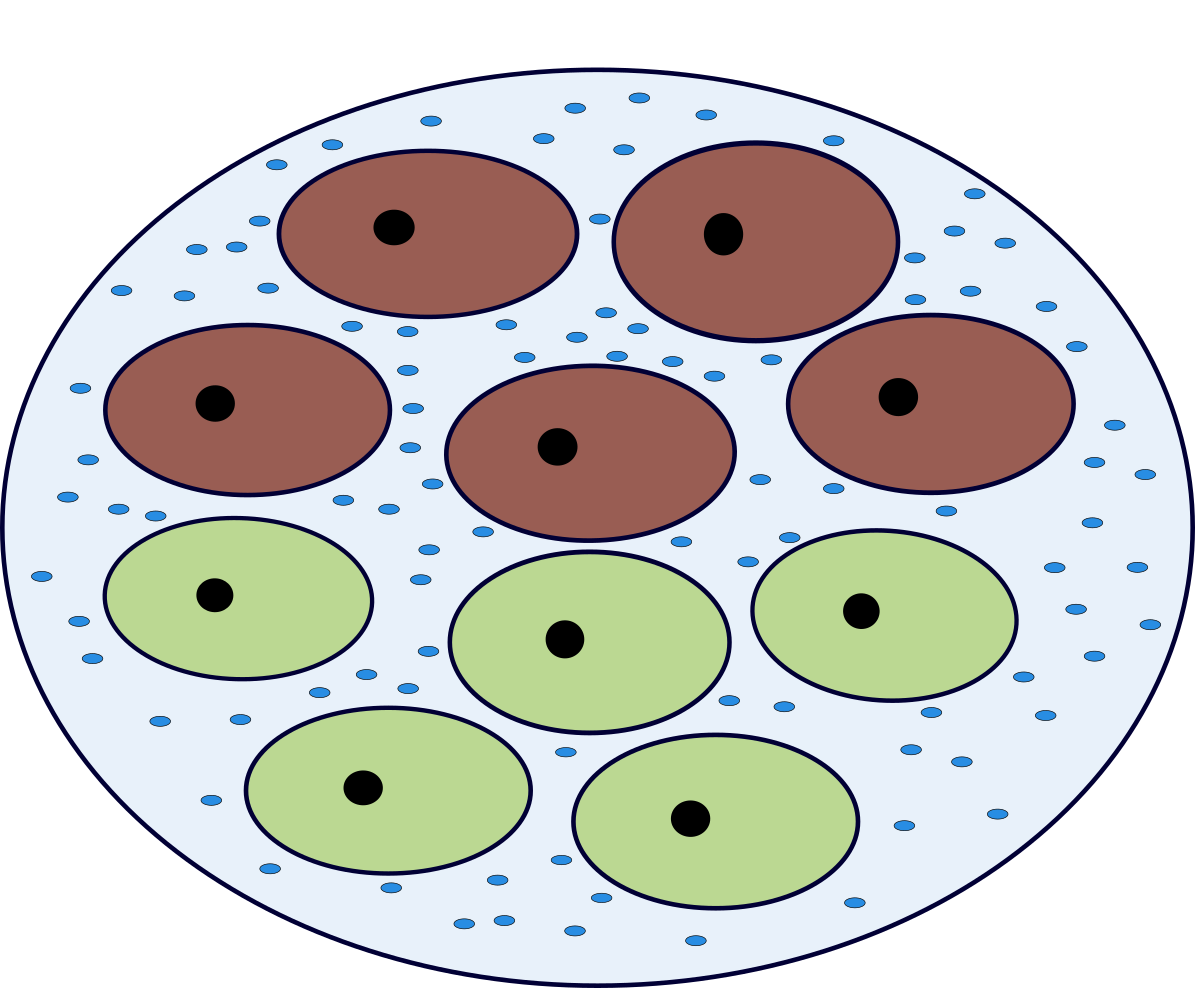
\includegraphics[scale=0.1]{img/celulas.png}
		\caption{Interacción entre las cuatro especies.}
	\end{figure}
	Variables $\alert{u}$ y $\alert{n}$ con valores en [0,1]:
	\begin{itemize}
		\item $u$ de tipo campo de fase ($1$ células tumorales y $0$ células sanas).
		\item $n$ porcentaje de nutrientes en el agua extracelular.
	\end{itemize}

%	\structure{\textbf{energía}} $E\colon H^1(\Omega)\times H^1(\Omega)\longrightarrow\R$ se define como 
%	\begin{align*}
%	E(u(t),n(t))&\coloneqq\int_\Omega\left(\frac{\varepsilon^2}{2}|\nabla u(x,t)|^2+F(u(x,t))-\chi_0u(x,t)n(x,t)+\frac{1}{2\delta}\left(n(x,t)\right)^2\right)dx.
%	\end{align*}
\end{frame}

\begin{frame}{Modelo de tumores}
	\footnotesize
	\begin{block}{}
		\vspace*{-0.4cm}
		\begin{equation*}
			\left\{\begin{aligned}
			\partial_t u&=\nabla\cdot\left(M_u\nabla \left(F'(u)-\varepsilon^2\Delta u\right)\right) \framedmath<2>{-\chi_0\nabla\cdot\left(M_u\nabla n\right)}\notag\\&\quad\framedmath<3>{+\delta P_0 u_+(\mu_n-\mu_u)}\quad&\text{en }\Omega\times (0,T),\\
			\partial_t n&=\frac{1}{\delta}\nabla\cdot\left(M_n\nabla n \right)\framedmath<2>{-\chi_0\nabla\cdot \left(M_n\nabla u \right)}\notag\\&\quad\framedmath<3>{-\delta P_0 u_+(\mu_n-\mu_u)}\quad&\text{en }\Omega\times (0,T),\\
			\nabla u\cdot \mathbf{n}&=\nabla n\cdot \mathbf{n}=\nabla \mu_u\cdot \mathbf{n}=0 \quad &\text{sobre }\partial\Omega\times (0,T),\\
			u(0)&=u_0,\quad n(0)=n_0\quad&\text{en }\Omega,
			\end{aligned}\right.
		\end{equation*}
	\end{block}
	donde $u_0,n_0\in L^2(\Omega)$ son las condiciones iniciales.
	
	\vspace*{0.3cm}
	\begin{itemize}
		\item $\alert{F(u)}=\Gamma u^2(1-u)^2,$ \alert{$\Gamma>0$} funcional de doble pozo Ginzburg-Landau.
		\item $\alert{\mu_u}=F'(u)-\varepsilon^2\Delta u+\partial_u\chi(u,n)$ potencial químico de $u$.
		\item $\alert{\mu_n}=\frac{1}{\delta} n + \partial_n\chi(u,n)$ potencial químico de $n$.
		\item<2> \myframed{Desplazamiento de células tumorales $\longleftarrow$ \textbf{Términos de difusión cruzada}.}
		\item<3> \myframed{Reacciones químicas células-nutrientes.}
	\end{itemize}
	
\end{frame}

\begin{frame}{Crecimiento de un tumor con fuente de nutrientes}
	
	\begin{figure}[H]
%		\vspace*{-0.6cm}
		\begin{subfigure}{0.49\textwidth}
			\centering
			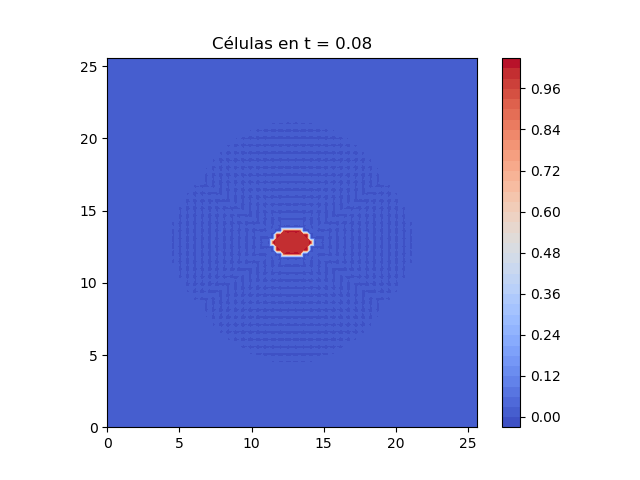
\includegraphics[scale=0.3]{img/Tumor-Model_tests/Test2_revision/u_FEM-Eyre-nestac-revision_nt-1000_t-0.0800_P1_nx-100_elipse-1.7-0.9.png}
		\end{subfigure}
		\hspace*{-1.5cm}
		\begin{subfigure}{0.49\textwidth}
			\centering
			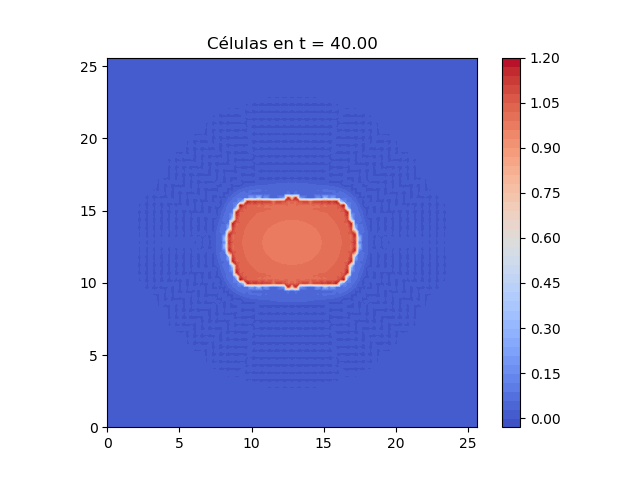
\includegraphics[scale=0.3]{img/Tumor-Model_tests/Test2_revision/u_FEM-Eyre-nestac-revision_nt-1000_t-40.0000_P1_nx-100_elipse-1.7-0.9.png}
		\end{subfigure}
		\begin{subfigure}{0.49\textwidth}
			\centering
			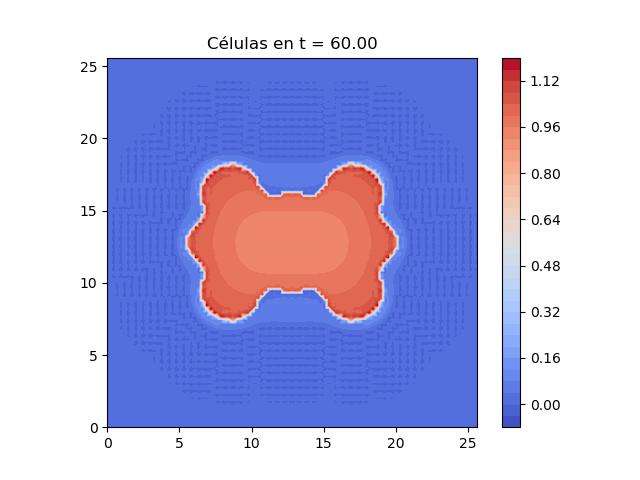
\includegraphics[scale=0.3]{img/Tumor-Model_tests/Test2_revision/u_FEM-Eyre-nestac-revision_nt-1000_t-60.0000_P1_nx-100_elipse-1.7-0.9.png}
		\end{subfigure}
		\hspace*{-1.5cm}
		\begin{subfigure}{0.49\textwidth}
			\centering
			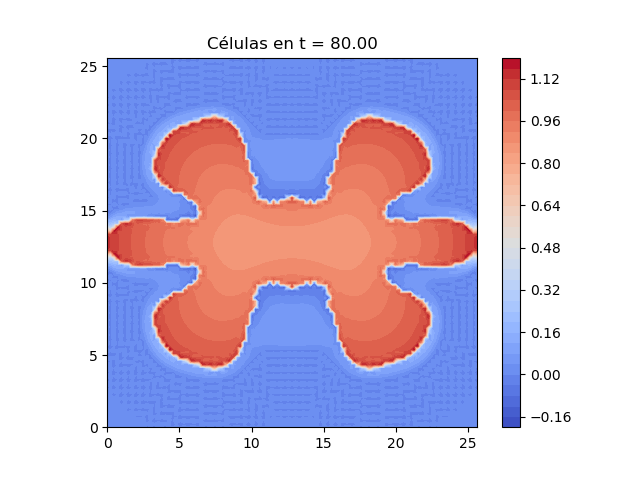
\includegraphics[scale=0.3]{img/Tumor-Model_tests/Test2_revision/u_FEM-Eyre-nestac-revision_nt-1000_t-80.0000_P1_nx-100_elipse-1.7-0.9.png}
		\end{subfigure}
		%\caption{Representación de las células para la solución obtenida.}
		\begin{center}
			\vspace*{-0.3cm}
			\scriptsize{\structure{Figura:} Representación de las células para la solución obtenida.}
		\end{center}
	\end{figure}
	
\end{frame}

\begin{frame}{Agregación de tumores circulares}
		\begin{figure}[H]
%		\vspace*{-0.6cm}
		\begin{subfigure}{0.49\textwidth}
			\centering
			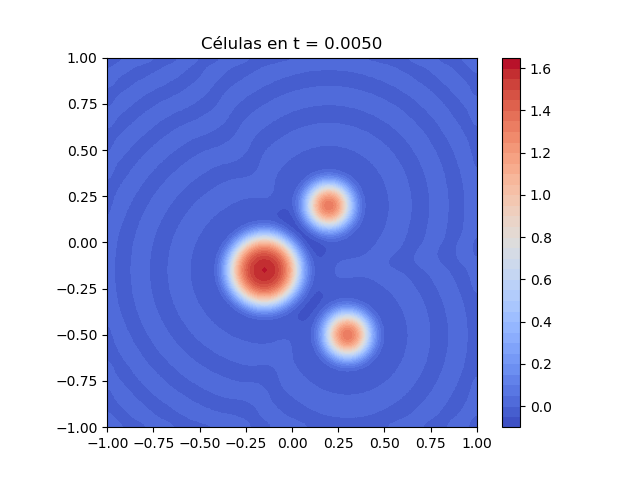
\includegraphics[scale=0.3]{img/Tumor-Model_tests/Test4/u_DG-EQ-3tumors_nt-1000_t-0.0050_P1_nx-120_P0-100.png}
		\end{subfigure}
		\hspace*{-1.5cm}
		\begin{subfigure}{0.49\textwidth}
			\centering
			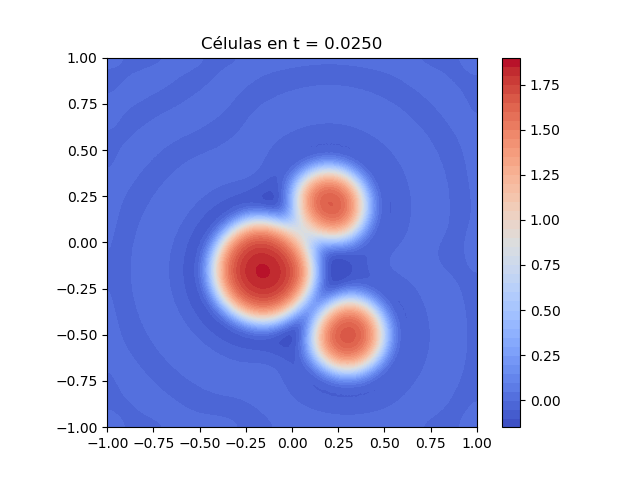
\includegraphics[scale=0.3]{img/Tumor-Model_tests/Test4/u_DG-EQ-3tumors_nt-1000_t-0.0250_P1_nx-120_P0-100.png}
		\end{subfigure}
		\begin{subfigure}{0.49\textwidth}
			\centering
			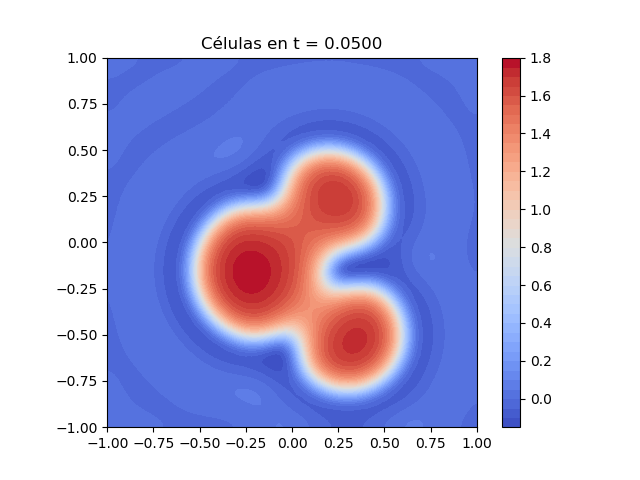
\includegraphics[scale=0.3]{img/Tumor-Model_tests/Test4/u_DG-EQ-3tumors_nt-1000_t-0.0500_P1_nx-120_P0-100.png}
		\end{subfigure}
		\hspace*{-1.5cm}
		\begin{subfigure}{0.49\textwidth}
			\centering
			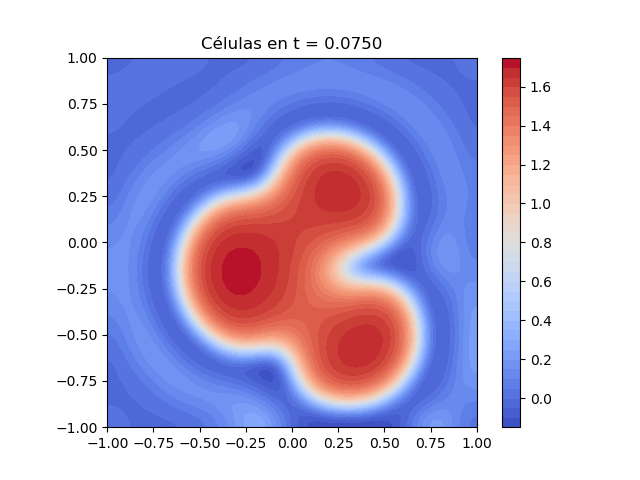
\includegraphics[scale=0.3]{img/Tumor-Model_tests/Test4/u_DG-EQ-3tumors_nt-1000_t-0.0750_P1_nx-120_P0-100.png}
		\end{subfigure}
		%		\caption{Representación de las células en diferentes instantes de tiempo.}
		\begin{center}
			\vspace*{-0.3cm}
			\scriptsize{\structure{Figura:} Representación de las células para la solución obtenida.}
		\end{center}
	\end{figure}
\end{frame}

\subsubsection{Modelos de migración celular}

\begin{frame}{Modelo de migración celular}
	\begin{figure}[H]
	\centering
	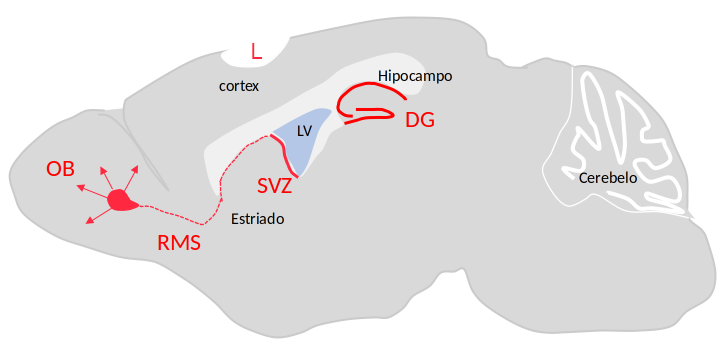
\includegraphics[scale=0.4]{img/Esquema_cerebro_Modelos.png}
	\caption{Esquema del movimiento de los neuroblastos por el cerebro de un roedor.}
	\end{figure}
\end{frame}

\section{Resolución matemática}

\subsection{Problema elíptico}

\begin{frame}{Problema modelo}
	Consideramos el problema de Poisson:
	\begin{block}{}
		\begin{equation*}
		\label{prob_modelo_Poisson}
		\left\{
		\begin{aligned}
		-\Delta u&=f & \text{en } &\Omega, \\
		u&=0 & \text{en } &\partial\Omega,
		\end{aligned}
		\right.
		\end{equation*}
	\end{block}
	donde $f\in L^2\left(\Omega\right)$.
\end{frame}

\begin{frame}{Formulación variacional continua}
	
	\textbf{Espacio de soluciones}: $\alert{H_0^1(\Omega)}$.
	\begin{itemize}\itemsep1em
		\item $a\colon H^1_0(\Omega)\times H_0^1(\Omega)\to\R$, $\displaystyle \alert{a(u,v)}\coloneqq\int_\Omega\nabla u\nabla v$;
		\item $L\colon H_0^1(\Omega)\to\R$, $\displaystyle \alert{L(v)}\coloneqq\int_\Omega f v$.
	\end{itemize}
	\textbf{Problema variacional}:
	\begin{block}{}
		\begin{center}
			\label{form_var_Poisson}
			$\text{encontrar } u\in H^1_0(\Omega) \text{ tal que } a(u,v)=L(v)\text{ para todo } v\in H_0^1(\Omega)$.
		\end{center}
	\end{block}
	
	\vspace*{1cm}
	El problema modelo y su formulación variacional son \alert{equivalentes}.
	
\end{frame}

\begin{frame}{Malla de $\bar{\Omega}$}
	
	Conjunto $\alert{\mathcal{T}_h}$ de $d$-símplices $\left(K_i\right)_{i\in\left\{1,2,\ldots,N_{\mathcal{T}_h}\right\}}$ no degenerados que satisfacen:
		\begin{itemize}
			\item $K_i\subseteq\bar\Omega$ para todo $i\in\left\{1,2,\ldots,N_{\mathcal{T}_h}\right\}$;
			\item $\text{int}\left(K_i\right)\cap\text{int}\left(K_j\right)=\varnothing$ para $i,j\in\left\{1,2,\ldots,N_{\mathcal{T}_h} \right\}$ con $i\neq j$;
			\item $\displaystyle \bigcup_{i=1}^{N_{\mathcal{T}_h}} K_i=\bar\Omega$.
		\end{itemize}
	
%	Generalmente $\mathcal{P}_i=\mathbb{P}_k$.
\vspace*{-0.2cm}
\begin{figure}[H]
	\centering
	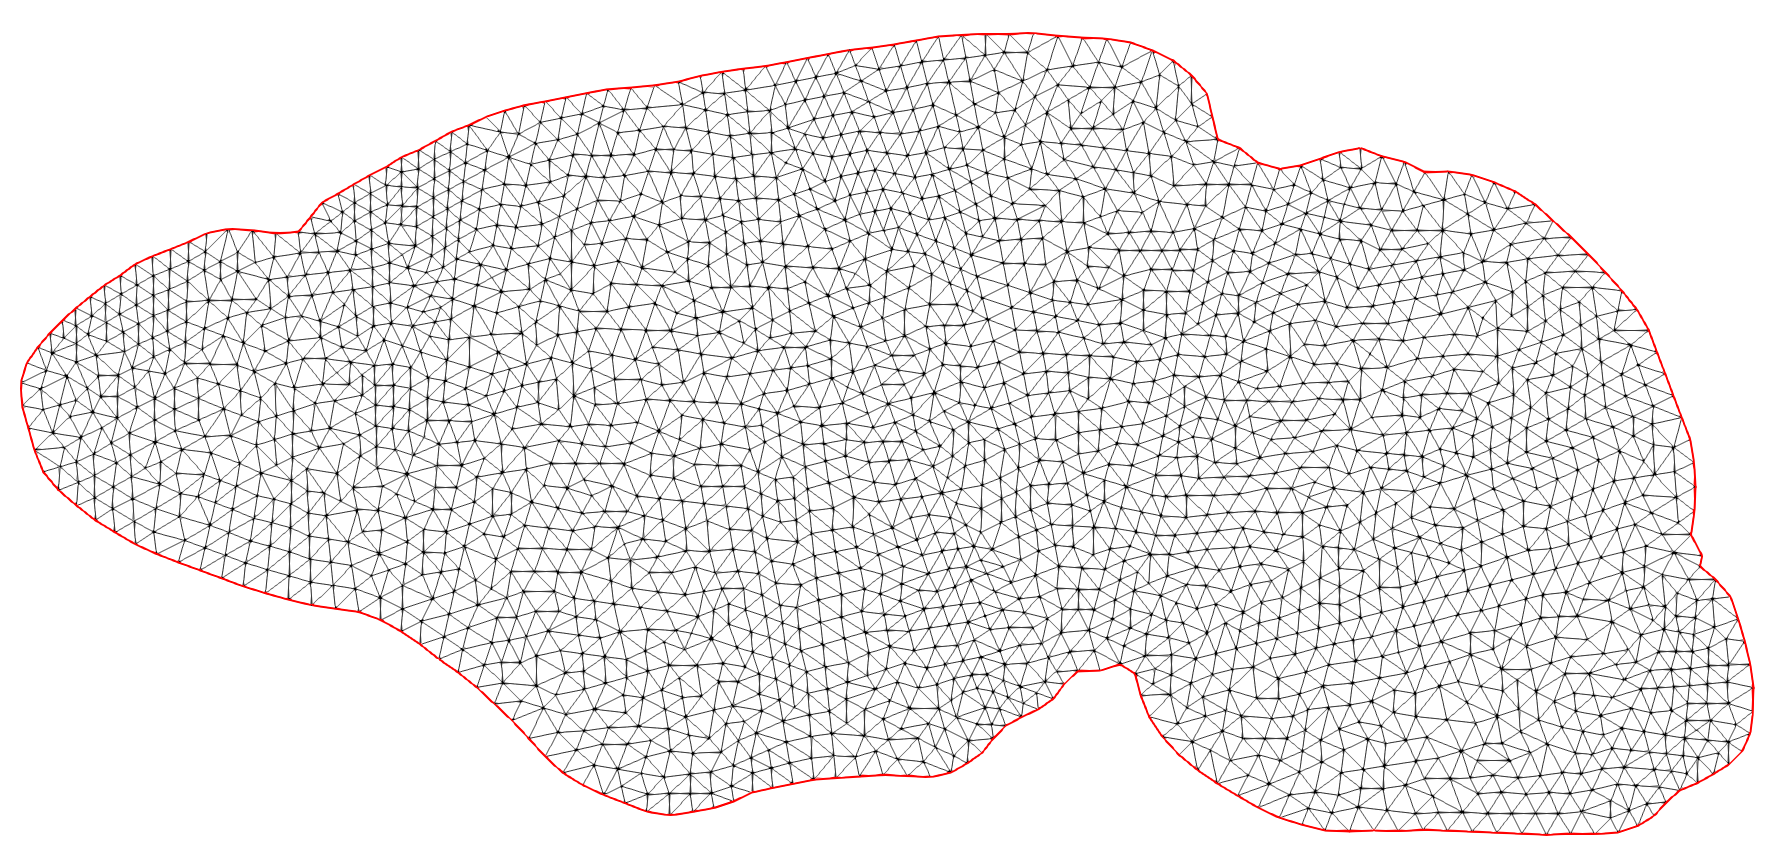
\includegraphics[scale=0.15]{img/malla_cerebro.png}
\end{figure}
	
\end{frame}

\begin{frame}{Aproximaciones discretas}
	
\textbf{Método de los Elementos Finitos:}
\begin{block}{}
	\begin{center}
		$\alert{V_h}\coloneqq\left\{v_h\in \mathcal{C}^0\left(\bar\Omega\right)\colon v_{h|_{K_i}}\in \mathbb{P}_k(K_i) \text{ con } K_i\in\mathcal{T}_h, \forall i\in\left\{1,2,\ldots,N_{\mathcal{T}_h} \right\}\right\}$
	\end{center}
\end{block}
con base $\left\{\varphi_i\right\}_{i\in\left\{1,2,\ldots,N_h \right\}}$.

\vspace*{1cm}
\textbf{Métodos de Galerkin discontinuos:}
\begin{block}{}
	\begin{center}
		$\alert{\S_h}\coloneqq\left\{v_h\in L^2(\Omega)\colon v_{h|_{K_i}}\in\mathbb{P}_k(K_i)\text{ con } K_i\in\T_h,\forall i\in\left\{1,2,\ldots,N_{\T_h}\right\}\right\}$
	\end{center}
\end{block}
con base $\left\{\phi_i\right\}_{i\in\left\{1,2,\ldots,N_h \right\}}$.

\end{frame}

\begin{frame}{Método de los Elementos Finitos}
\vspace*{-0.3cm}
\begin{itemize}
	\item Encontrar $u\in V$ tal que $a(u,v)=L(v)$ para todo $v\in V$.
\end{itemize}
\vspace*{0.1cm}
$$\Big{\downarrow}$$
\vspace*{-0.3cm}
\begin{itemize}
	\item Encontrar $u_h\in V_h$ tal que $a(u_h,v_h)=L(v_h)$ para todo $v_h\in V_h$.
\end{itemize}
\vspace*{0.1cm}
$$\Big{\Updownarrow}$$
\vspace*{-0.3cm}
\begin{itemize}
	\item Resolver el sistema lineal $A\mathbf{U}=\mathbf{F}$ donde:
	\vspace*{0.3cm}
	\begin{itemize}
		\item $A=\left(A_{i j}\right)_{i, j\in\left\{1,2,\ldots,N_h\right\}}$ con $A_{i j}=a(\varphi_j,\varphi_i)$;
		\item $\mathbf{U}=\left(U_1,U_2,\ldots,U_{N_h}\right)^t$ con $u_h=\displaystyle\sum_{i=1}^{N_h}U_i\varphi_i$;
		\item $\mathbf{F}=\left(F_1,F_2,\ldots,F_{N_h}\right)^t$ con $F_i=L\left(\varphi_i\right)$.
	\end{itemize}
\end{itemize}
\end{frame}

\begin{frame}{Método de Galerkin discontinuo}
	
	\onslide<1>{\textbf{Primera idea:}}
	\begin{itemize}
		\item<1> Encontrar $u\in V$ tal que $a(u,v)=L(v)$ para todo $v\in V$.
	\end{itemize}
	\vspace*{0.1cm}
	\onslide<1>{$$\Big{\downarrow}\longleftarrow\text{\alert{¡ERROR!}}$$}
	\vspace*{-0.3cm}
	\begin{itemize}
		\item<1> Encontrar $u_h\in \S_h$ tal que $a(u_h,v_h)=L(v_h)$ para todo $v_h\in \S_h$.
	\end{itemize}

	\vspace*{1cm}
	\onslide<2>{\textbf{Idea correcta:}}
	\begin{itemize}
		\item<2> Encontrar $u\in V$ tal que $a(u,v)=L(v)$ para todo $v\in V$.
	\end{itemize}
	\vspace*{0.1cm}
	\onslide<2>{$$\Big{\downarrow}$$}
	\vspace*{-0.3cm}
	\begin{itemize}
		\item<2> Encontrar $u_h\in\S_h$ tal que $\asip{u_h}{v_h}=L(v_h)$ para todo $v_h\in \S_h$.
	\end{itemize}
	
\end{frame}

\begin{frame}{Forma bilineal SIP}
	\begin{itemize}\itemsep1em
		\item $a_h^{\text{sip}}:\S_{*h}\times \S_h\to\R$,
		\begin{equation*}
		\label{forma_bilineal_DG}
		\begin{aligned}
		\alert{\asip{u}{v_h}}&\coloneqq \framedmath<2>{\displaystyle \sum_{K\in\T_h}\int_K\nabla_h u\nabla_h v-\sum_{e\in\E_h}\int_e\media{\nabla_h u\cdot\mathbf{n}_e}\salto{v_h}}\\&\framedmath<3>{\displaystyle -\sum_{e\in\E_h}\int_e\media{\nabla_h v\cdot\mathbf{n}_e}\salto{u}}\\&\framedmath<4>{\displaystyle +\sigma\sum_{e\in\E_h}\int_e\frac{1}{h_e}\salto{u}\salto{v_h}};
		\end{aligned}
		\end{equation*}
		\begin{itemize}
			\item<2> \myframed{Fórmula de integracion por partes}
			\item<3> \myframed{Simetría}
			\item<4> \myframed{Coercitividad}
		\end{itemize}
		\item $L_h:\S_h\to\R$, $\displaystyle \alert{L_h(v_h)}\coloneqq \int_\Omega f v_h.$
	\end{itemize}
	
\end{frame}

\begin{frame}{Método de Penalización Interior Simétrica}
	\vspace*{-0.3cm}
	\begin{itemize}
		\item Encontrar $u\in V$ tal que $a(u,v)=L(v)$ para todo $v\in V$.
	\end{itemize}
	\vspace*{0.1cm}
	$$\Big{\downarrow}$$
	\vspace*{-0.3cm}
	\begin{itemize}
		\item $\text{Encontrar }u_h\in\S_h\text{ tal que }\asip{u_h}{v_h}=L_h(v_h)\text{ para todo }v_h\in\S_h.$
	\end{itemize}
	\vspace*{0.1cm}
	$$\Big{\Updownarrow}$$
	\vspace*{-0.3cm}
	\begin{itemize}
		\item Resolver el sistema lineal $A^{\text{sip}}\mathbf{U}^{\text{sip}}=\mathbf{F}^{\text{sip}}$ donde:
		\vspace*{0.3cm}
		\begin{itemize}
			\item $A^{\text{sip}}=\left(A_{ij}^{\text{sip}}\right)_{i,j\in\left\{1,2,\ldots,N_h^{\text{sip}}\right\}}$ con $A_{ij}^{\text{sip}}=\asip{\phi_j}{\phi_i}$;
			\item $\mathbf{U}^{\text{sip}}=\left(U_1^{\text{sip}},U_2^{\text{sip}},\ldots,U_{N_h^{\text{sip}}}^{\text{sip}}\right)^t$ con $u_h=\displaystyle\sum_{i=1}^{N_h^{\text{sip}}}U_i^{\text{sip}}\phi_i$;
			\item $\mathbf{F}^{\text{sip}}=\left(F_1^{\text{sip}},F_2^{\text{sip}},\ldots,F_{N_h^{\text{sip}}}^{\text{sip}}\right)^t$ con $F_i^{\text{sip}}=L_h(\phi_i)$.
		\end{itemize}
	\end{itemize}
\end{frame}

\begin{frame}{Soluciones numéricas}
	\begin{figure}[h!]
		\begin{subfigure}[b]{0.215\textwidth}
			\centering
			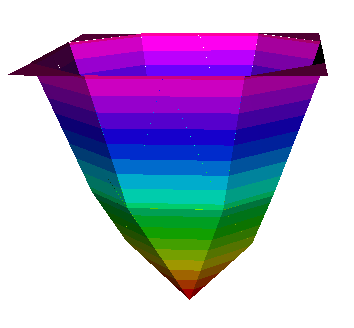
\includegraphics[scale=0.16]{img/Difusion/Recortes/steady_diffusion_exact_n_4.png}
			\caption{Solución exacta.}
		\end{subfigure}
		\begin{subfigure}[b]{0.215\textwidth}
			\centering
			
\includegraphics[scale=0.16]{img/Difusion/Recortes/steady_diffusion_approx_n_4.png}
			\caption{Solución discreta.}
		\end{subfigure}
		\begin{subfigure}[b]{0.11\textwidth}
			\centering
			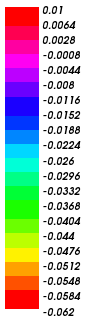
\includegraphics[scale=0.23]{img/Difusion/Recortes/steady_diffusion_values.png}
			%\caption*{ }
		\end{subfigure}
		\begin{subfigure}[b]{0.215\textwidth}
			\centering
			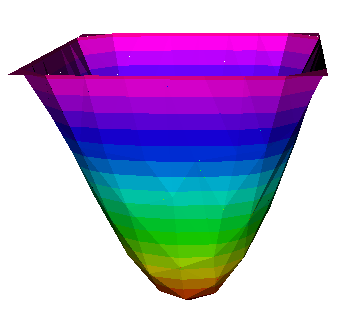
\includegraphics[scale=0.16]{img/Difusion/Recortes/steady_diffusion_exact_n_8.png}
			\caption{Solución exacta.}
		\end{subfigure}
		\begin{subfigure}[b]{0.215\textwidth}
			\centering
			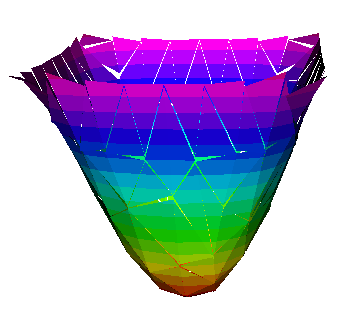
\includegraphics[scale=0.16]{img/Difusion/Recortes/steady_diffusion_approx_n_8.png}
			\caption{Solución discreta.}
		\end{subfigure}
		\caption{A la izquierda $h\approx\frac{1}{4}$. A la derecha $h\approx\frac{1}{8}$.}
	\end{figure}
	\begin{figure}[h!]
		\begin{subfigure}[b]{0.215\textwidth}
			\centering
			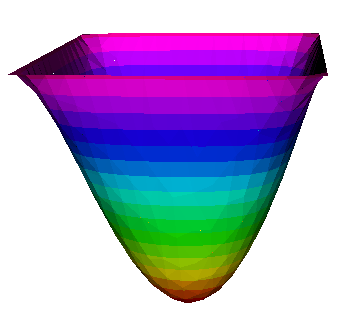
\includegraphics[scale=0.16]{img/Difusion/Recortes/steady_diffusion_exact_n_16.png}
			\caption{Solución exacta.}
		\end{subfigure}
		\begin{subfigure}[b]{0.215\textwidth}
			\centering
			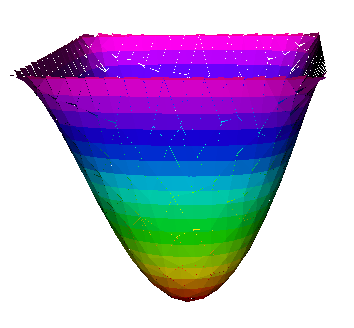
\includegraphics[scale=0.16]{img/Difusion/Recortes/steady_diffusion_approx_n_16.png}
			\caption{Solución discreta.}
		\end{subfigure}
		\begin{subfigure}[b]{0.11\textwidth}
			\centering
			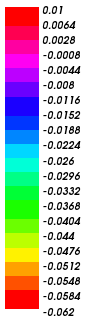
\includegraphics[scale=0.23]{img/Difusion/Recortes/steady_diffusion_values.png}
			%\caption*{ }
		\end{subfigure}
		\begin{subfigure}[b]{0.215\textwidth}
			\centering
			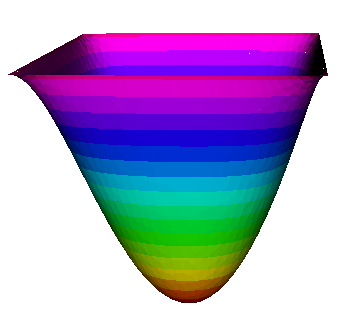
\includegraphics[scale=0.16]{img/Difusion/Recortes/steady_diffusion_exact_n_32.png}
			\caption{Solución exacta.}
		\end{subfigure}
		\begin{subfigure}[b]{0.215\textwidth}
			\centering
			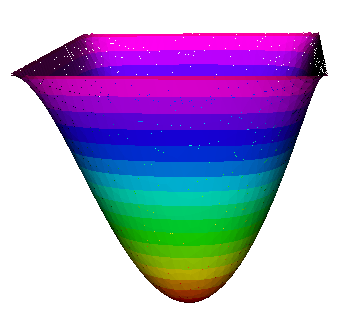
\includegraphics[scale=0.16]{img/Difusion/Recortes/steady_diffusion_approx_n_32.png}
			\caption{Solución discreta.}
		\end{subfigure}
		\caption{A la izquierda $h\approx\frac{1}{16}$. A la derecha $h\approx\frac{1}{32}$.}
	\end{figure}
\end{frame}

\subsection{Problema hiperbólico}

\begin{frame}{Problema modelo}
	Consideramos el problema de convección-reacción:
	\begin{block}{}
		\begin{equation*}
		\label{prob_modelo_hiperbolica}
		\left\{
		\begin{aligned}
		\beta\cdot\nabla u+\mu u&=f & \text{en } &\Omega, \\
		u&=0 & \text{en } &\partial\Omega^-,
		\end{aligned}
		\right.
		\end{equation*}
	\end{block}
	donde 
	\begin{itemize}
		\item $\partial\Omega^-=\left\{x\in\partial\Omega\colon \beta(x)\mathbf{n}(x)<0\right\},$
		\item $\mu\in L^\infty(\Omega)$,
		\item $\beta\in\left[\text{Lip}(\Omega)\right]^d$,
		\item $f\in L^2(\Omega)$.
	\end{itemize}
	\vspace*{.5cm}
	Asumimos que existe $\mu_0>0$ tal que $\displaystyle\mu-\frac{1}{2}\nabla\cdot\beta\geq\mu_0$ en $\Omega$.
	
\end{frame}

\begin{frame}{Formulación variacional continua}
	\textbf{Espacio de soluciones}: $\alert{V}$ (espacio de los grafos).
	\begin{itemize}\itemsep1em
		\item $a\colon V\times V\to \R$, $$\alert{a(u,v)}\coloneqq\int_\Omega(\beta\cdot\nabla u)v+\int_\Omega\mu u v+\int_{\partial\Omega}(\beta\mathbf{n})^-uv;$$
		\item $L\colon V\to\R$, $$\alert{L(v)}\coloneqq\int_\Omega f v.$$
	\end{itemize}
	\textbf{Problema variacional}:
	\begin{block}{}
		\begin{center}
			$\text{encontrar }u\in V\text{ tal que }a(u,v)=L(v)\text{ para todo } v\in V.$
		\end{center}
	\end{block}
	
	\begin{itemize}\itemsep1em
		\item El problema modelo y su formulación variacional son \alert{equivalentes} en $V$.
		
		\item Existe solución y es única.
	\end{itemize}
	
\end{frame}

\begin{frame}{Métodos de flujos}
	\vspace*{-0.3cm}
	\begin{itemize}
		\item Encontrar $u\in V$ tal que $a(u,v)=L(v)$ para todo $v\in V$.
	\end{itemize}
	\vspace*{0.1cm}
	$$\Big{\downarrow}$$
	\vspace*{-0.3cm}
	\begin{itemize}
		\item $\text{Encontrar }u_h\in \S_h\text{ tal que }\adg{u_h}{v_h}=L_h(v_h)\text{ para todo }v_h\in \S_h$.
	\end{itemize}
	\vspace*{0.1cm}
	$$\Big{\Updownarrow}$$
	\vspace*{-0.3cm}
	\begin{itemize}
		\item Resolver el sistema lineal $A^{\text{DG}}\mathbf{U}^{\text{DG}}=\mathbf{F}^{\text{DG}}$ donde:
		\vspace*{0.3cm}
		\begin{itemize}
			\item $A^{\text{DG}}=\left(A_{ij}^{\text{DG}}\right)_{i,j\in\left\{1,2,\ldots,N_h^{\text{upw}}\right\}}$ con $A_{ij}^{\text{DG}}=\adg{\phi_j}{\phi_i}$;
			\item $\mathbf{U}^{\text{DG}}=\left(U_1^{\text{DG}},U_2^{\text{DG}},\ldots,U_{N_h^{\text{DG}}}^{\text{DG}}\right)^t$ con $u_h=\displaystyle\sum_{i=1}^{N_h^{\text{DG}}}U_i^{\text{DG}}\phi_i$;
			\item $\mathbf{F}^{\text{DG}}=\left(F_1^{\text{DG}},F_2^{\text{DG}},\ldots,F_{N_h^{\text{DG}}}^{\text{DG}}\right)^t$ con $F_i^{\text{DG}}=L_h(\phi_i)$.
		\end{itemize}
\end{itemize}

\vspace*{0.3cm}
\footnotesize
Donde $\adg{u_h}{v_h}=\alert{\acf{u_h}{v_h}}\text{ (\structure{flujos centrados})  o }\alert{\aupw{u_h}{v_h}}\text{ (\structure{flujos aguas arriba})}$.

\end{frame}

\begin{frame}{Soluciones numéricas}
	\vspace{-0.1cm}
	\begin{figure}[h!]
		\begin{subfigure}[b]{0.27\textwidth}
			\centering
			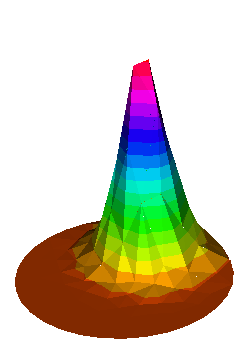
\includegraphics[scale=0.22]{img/Conveccion_Reaccion/Recortes/steady_convect_react_exact_n_32.png}
			\caption{Solución exacta.}
		\end{subfigure}
		\begin{subfigure}[b]{0.27\textwidth}
			\centering
			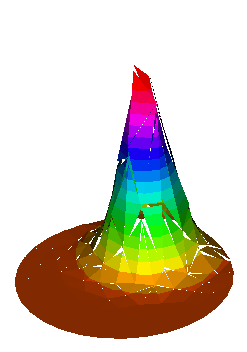
\includegraphics[scale=0.22]{img/Conveccion_Reaccion/Recortes/steady_convect_react_approx_CF_n_32.png}
			\caption{Flujos Centrados.}
		\end{subfigure}
		\begin{subfigure}[b]{0.27\textwidth}
			\centering
			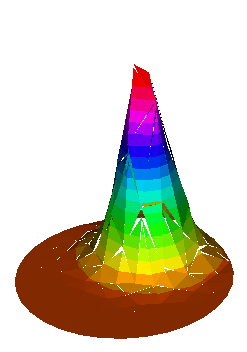
\includegraphics[scale=0.22]{img/Conveccion_Reaccion/Recortes/steady_convect_react_approx_UPW_n_32.png}
			\caption{Aguas Arriba.}
		\end{subfigure}
		\begin{subfigure}[b]{0.15\textwidth}
			\centering
			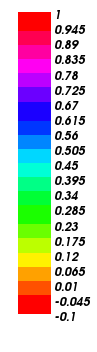
\includegraphics[scale=0.22]{img/Conveccion_Reaccion/Recortes/steady_convect_react_values.png}
			%\caption*{ }
		\end{subfigure}
		\caption{Gráficas obtenidas con $h\approx\frac{\pi}{16}$.}
	\end{figure}
	\vspace{-0.55cm}
	\begin{figure}[h!]
		\begin{subfigure}[b]{0.27\textwidth}
			\centering
			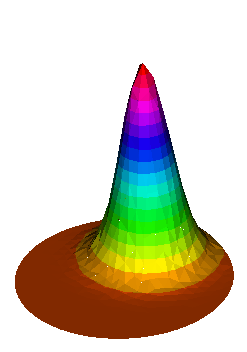
\includegraphics[scale=0.22]{img/Conveccion_Reaccion/Recortes/steady_convect_react_exact_n_64.png}
			\caption{Solución exacta.}
		\end{subfigure}
		\begin{subfigure}[b]{0.27\textwidth}
			\centering
			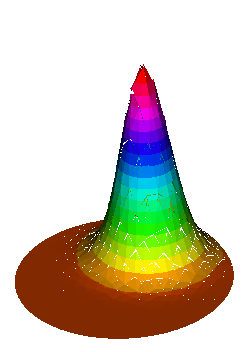
\includegraphics[scale=0.22]{img/Conveccion_Reaccion/Recortes/steady_convect_react_approx_CF_n_64.png}
			\caption{Flujos Centrados.}
		\end{subfigure}
		\begin{subfigure}[b]{0.27\textwidth}
			\centering
			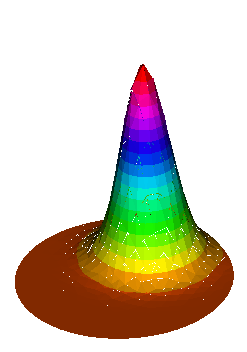
\includegraphics[scale=0.22]{img/Conveccion_Reaccion/Recortes/steady_convect_react_approx_UPW_n_64.png}
			\caption{Aguas Arriba.}
		\end{subfigure}
		\begin{subfigure}[b]{0.15\textwidth}
			\centering
			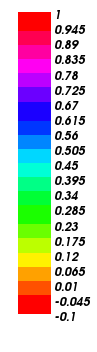
\includegraphics[scale=0.22]{img/Conveccion_Reaccion/Recortes/steady_convect_react_values.png}
			%\caption*{ }
		\end{subfigure}
		\caption{Gráficas obtenidas con $h\approx\frac{\pi}{32}$.}
	\end{figure}
\end{frame}

%\subsection{Problema de convección-difusión evolutivo}

%\begin{frame}{INCLUIR VÍDEO}
%	\Huge\textbf{INCLUIR VÍDEO HIPERBÓLICO}
%\end{frame}

%\section{Bibliografía básica}

%\begin{frame}{Bibliografía básica}
%\vspace*{-0.1cm}
%\nocite*
%\bibliographystyle{plain}
%\bibliography{bibliografia}
%\end{frame}

\begin{frame}{}
\vspace*{3cm}
\begin{center}
\Huge
\emph{¡Gracias por su atención!}
\end{center}


\vspace*{2cm}
\footnotesize\color{darkgray}
Imágenes sobre el clima utilizadas:
\begin{enumerate}
	\footnotesize\color{darkgray}
	\item Madrid 264 weather girl. David Holt, licencia CC-by-sa.
	\item Isobaras. MediaCommons, User:Asierog, licencia CC-by-sa.
	\item NOAAWavewatch III 120-hour wind and wave forecast for the North Atlantic. Public domain.
\end{enumerate}

\end{frame}

\end{document}


%%% Local Variables:
%%% coding: utf-8
%%% TeX-master: t
%%% mode: latex
%%% ispell-local-dictionary: "english"
